\section{Ergebnisse Nutzerbefragung}

\textcolor{blue}{\textit{einleitende Worte}} \\

% Boxplots
\textcolor{red}{Titel ändern!}
\begin{figure}[H]
    \centering
    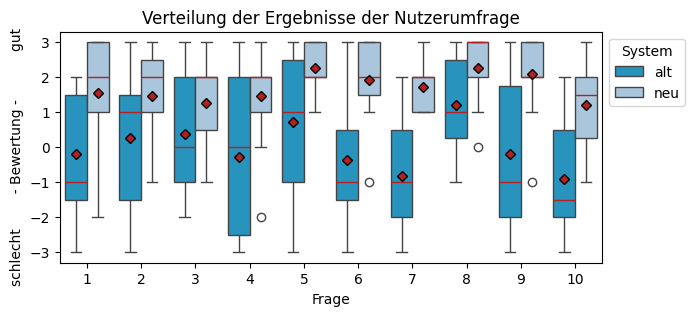
\includegraphics[width=1\linewidth]{Diagramme/pruemper_all.png}
    \caption{Auswertung der Fragen nach ISO 9241-110}
    \label{fig:pruemper_all}
\end{figure}

% Tabelle
\begin{table}[]
\begin{tabular}{|l|c|c|c|}
\hline
Frage 1   & $\Bar{x}$ & $\Tilde{x}$ & $\sigma$ \\ \hline
alt       & -0,2      & -1          & 1,75     \\ \hline
neu       & 1,55      & 2           & 1,5      \\ \hline
Differenz & +1,75     & +3          & -        \\ \hline
\end{tabular}
\begin{tabular}{|l|c|c|c|}
\hline
Frage 2   & $\Bar{x}$ & $\Tilde{x}$ & $\sigma$ \\ \hline
alt       & xxxx      &  xx         &  xxxx    \\ \hline
neu       & xxxx      &  xx         &  xxxx    \\ \hline
Differenz &           &             & -        \\ \hline
\end{tabular}
\begin{tabular}{|l|c|c|c|}
\hline
Frage 3   & $\Bar{x}$ & $\Tilde{x}$ & $\sigma$ \\ \hline
alt       & xxxx      &  xx         &  xxxx    \\ \hline
neu       & xxxx      &  xx         &  xxxx    \\ \hline
Differenz &           &             & -        \\ \hline
\end{tabular}
\begin{tabular}{|l|c|c|c|}
\hline
Frage 4   & $\Bar{x}$ & $\Tilde{x}$ & $\sigma$ \\ \hline
alt       & xxxx      &  xx         &  xxxx    \\ \hline
neu       & xxxx      &  xx         &  xxxx    \\ \hline
Differenz &           &             & -        \\ \hline
\end{tabular}
\begin{tabular}{|l|c|c|c|}
\hline
Frage 5   & $\Bar{x}$ & $\Tilde{x}$ & $\sigma$ \\ \hline
alt       & xxxx      &  xx         &  xxxx    \\ \hline
neu       & xxxx      &  xx         &  xxxx    \\ \hline
Differenz &           &             & -        \\ \hline
\end{tabular}
\begin{tabular}{|l|c|c|c|}
\hline
Frage 6   & $\Bar{x}$ & $\Tilde{x}$ & $\sigma$ \\ \hline
alt       & xxxx      &  xx         &  xxxx    \\ \hline
neu       & xxxx      &  xx         &  xxxx    \\ \hline
Differenz &           &             & -        \\ \hline
\end{tabular}
\begin{tabular}{|l|c|c|c|}
\hline
Frage 7   & $\Bar{x}$ & $\Tilde{x}$ & $\sigma$ \\ \hline
alt       & xxxx      &  xx         &  xxxx    \\ \hline
neu       & xxxx      &  xx         &  xxxx    \\ \hline
Differenz &           &             & -        \\ \hline
\end{tabular}
\begin{tabular}{|l|c|c|c|}
\hline
Frage 8   & $\Bar{x}$ & $\Tilde{x}$ & $\sigma$ \\ \hline
alt       & xxxx      &  xx         &  xxxx    \\ \hline
neu       & xxxx      &  xx         &  xxxx    \\ \hline
Differenz &           &             & -        \\ \hline
\end{tabular}
\begin{tabular}{|l|c|c|c|}
\hline
Frage 9   & $\Bar{x}$ & $\Tilde{x}$ & $\sigma$ \\ \hline
alt       & xxxx      &  xx         &  xxxx    \\ \hline
neu       & xxxx      &  xx         &  xxxx    \\ \hline
Differenz &           &             & -        \\ \hline
\end{tabular}
\begin{tabular}{|l|c|c|c|}
\hline
Frage 10   & $\Bar{x}$ & $\Tilde{x}$ & $\sigma$ \\ \hline
alt       & xxxx      &  xx         &  xxxx    \\ \hline
neu       & xxxx      &  xx         &  xxxx    \\ \hline
Differenz &           &             & -        \\ \hline
\end{tabular}
\begin{tabular}{ll}
\multicolumn{2}{l}{verwendete Formelzeichen:} \\ \hline
$\Bar{x}$          & Mittelwert               \\
$\Tilde{x}$        & Median                   \\
$\sigma$           & Standardabweichung      
\end{tabular}
\caption{Zusammenfassung der Ergebnisse der Nutzerumfrage (Weiterverarbeitung der Daten aus \autoref{tab:Nutzerbefragung:rohe_Daten})}
\label{tab:Nutzerbefragung:mittelwerte}
\end{table}

\begin{table}[H]
\begin{center}
\begin{tabular}{|l|c|c|c|c|c|}
\hline
Frage                                   & 1      & 2      & 3        & 4      & 5      \\ \hline
$\varnothing_{neu} - \varnothing_{alt}$ & 1,73   & 1,18   & 0,91     & 1,73   & 1,55   \\ \hline
T-Test                                  & 0,0195 & 0,0949 & 0,138729 & 0,0487 & 0,0231 \\ \hline
\end{tabular}
\begin{tabular}{|l|c|c|c|c|c|}
\hline
Frage                                   & 1      & 2      & 3        & 4      & 5      \\ \hline
$\varnothing_{neu} - \varnothing_{alt}$ & 1,73   & 1,18   & 0,91     & 1,73   & 1,55   \\ \hline
T-Test                                  & 0,0195 & 0,0949 & 0,138729 & 0,0487 & 0,0231 \\ \hline
\end{tabular}
\caption{Nutzerbefragung - Differenz der Antwortmittelwerte und T-Test-Ergebnisse (Weiterverarbeitung der Daten aus \autoref{tab:Nutzerbefragung:rohe_Daten})}
\label{tab:Nutzerbefragung:Differenz+ttest}
\end{center}
\end{table}


% ******************************************************************************************
%           Frage 2
% ******************************************************************************************
\noindent
Frage 2 - Die Software ist gut auf die Anforderungen der Arbeit zugeschnitten \\


% ******************************************************************************************
%           Frage 3
% ******************************************************************************************
\noindent
Frage 3 - Die Software ermöglicht einen leichten Wechsel zw. Menüs oder Masken \\


% ******************************************************************************************
%           Frage 4
% ******************************************************************************************
\noindent
Frage 4 - Die Software erleichtert die Orientierung durch eine einheitliche Gestaltung \\


% ******************************************************************************************
%           Frage 5
% ******************************************************************************************
\noindent
Frage 5 - Die Software lässt sich durchgehend nach einem einheitlichen Prinzip bedienen \\


% ******************************************************************************************
%           Frage 6
% ******************************************************************************************
\noindent
Frage 6 - Die Software erfordert wenig Zeit zum Erlernen \\


% ******************************************************************************************
%           Frage 7
% ******************************************************************************************
\noindent
Frage 7 - Die Software erfordert nicht, dass man sich viele Details merken muss \\


% ******************************************************************************************
%           Frage 8
% ******************************************************************************************
\noindent
Frage 8 - Die Software erfordert keine überflüssigen Eingaben \\


% ******************************************************************************************
%           Frage 9
% ******************************************************************************************
\noindent
Frage 9 - Die Software ist gut ohne fremde Hilfe oder Handbuch erlernbar \\


% ******************************************************************************************
%           Frage 10
% ******************************************************************************************
\noindent
Frage 10 - Die Software bietet von sich aus situationsspezifische Erklärungen, die Konkret weiterhelfen \\


\subsection{Fehlerbetrachtung}
- Fehlerhafte Daten